% Options for packages loaded elsewhere
\PassOptionsToPackage{unicode}{hyperref}
\PassOptionsToPackage{hyphens}{url}
\PassOptionsToPackage{dvipsnames,svgnames,x11names}{xcolor}
%
\documentclass[
  letterpaper,
  DIV=11,
  numbers=noendperiod]{scrartcl}

\usepackage{amsmath,amssymb}
\usepackage{iftex}
\ifPDFTeX
  \usepackage[T1]{fontenc}
  \usepackage[utf8]{inputenc}
  \usepackage{textcomp} % provide euro and other symbols
\else % if luatex or xetex
  \usepackage{unicode-math}
  \defaultfontfeatures{Scale=MatchLowercase}
  \defaultfontfeatures[\rmfamily]{Ligatures=TeX,Scale=1}
\fi
\usepackage{lmodern}
\ifPDFTeX\else  
    % xetex/luatex font selection
\fi
% Use upquote if available, for straight quotes in verbatim environments
\IfFileExists{upquote.sty}{\usepackage{upquote}}{}
\IfFileExists{microtype.sty}{% use microtype if available
  \usepackage[]{microtype}
  \UseMicrotypeSet[protrusion]{basicmath} % disable protrusion for tt fonts
}{}
\makeatletter
\@ifundefined{KOMAClassName}{% if non-KOMA class
  \IfFileExists{parskip.sty}{%
    \usepackage{parskip}
  }{% else
    \setlength{\parindent}{0pt}
    \setlength{\parskip}{6pt plus 2pt minus 1pt}}
}{% if KOMA class
  \KOMAoptions{parskip=half}}
\makeatother
\usepackage{xcolor}
\setlength{\emergencystretch}{3em} % prevent overfull lines
\setcounter{secnumdepth}{-\maxdimen} % remove section numbering
% Make \paragraph and \subparagraph free-standing
\ifx\paragraph\undefined\else
  \let\oldparagraph\paragraph
  \renewcommand{\paragraph}[1]{\oldparagraph{#1}\mbox{}}
\fi
\ifx\subparagraph\undefined\else
  \let\oldsubparagraph\subparagraph
  \renewcommand{\subparagraph}[1]{\oldsubparagraph{#1}\mbox{}}
\fi


\providecommand{\tightlist}{%
  \setlength{\itemsep}{0pt}\setlength{\parskip}{0pt}}\usepackage{longtable,booktabs,array}
\usepackage{calc} % for calculating minipage widths
% Correct order of tables after \paragraph or \subparagraph
\usepackage{etoolbox}
\makeatletter
\patchcmd\longtable{\par}{\if@noskipsec\mbox{}\fi\par}{}{}
\makeatother
% Allow footnotes in longtable head/foot
\IfFileExists{footnotehyper.sty}{\usepackage{footnotehyper}}{\usepackage{footnote}}
\makesavenoteenv{longtable}
\usepackage{graphicx}
\makeatletter
\def\maxwidth{\ifdim\Gin@nat@width>\linewidth\linewidth\else\Gin@nat@width\fi}
\def\maxheight{\ifdim\Gin@nat@height>\textheight\textheight\else\Gin@nat@height\fi}
\makeatother
% Scale images if necessary, so that they will not overflow the page
% margins by default, and it is still possible to overwrite the defaults
% using explicit options in \includegraphics[width, height, ...]{}
\setkeys{Gin}{width=\maxwidth,height=\maxheight,keepaspectratio}
% Set default figure placement to htbp
\makeatletter
\def\fps@figure{htbp}
\makeatother

\KOMAoption{captions}{tableheading}
\makeatletter
\@ifpackageloaded{caption}{}{\usepackage{caption}}
\AtBeginDocument{%
\ifdefined\contentsname
  \renewcommand*\contentsname{Table of contents}
\else
  \newcommand\contentsname{Table of contents}
\fi
\ifdefined\listfigurename
  \renewcommand*\listfigurename{List of Figures}
\else
  \newcommand\listfigurename{List of Figures}
\fi
\ifdefined\listtablename
  \renewcommand*\listtablename{List of Tables}
\else
  \newcommand\listtablename{List of Tables}
\fi
\ifdefined\figurename
  \renewcommand*\figurename{Figure}
\else
  \newcommand\figurename{Figure}
\fi
\ifdefined\tablename
  \renewcommand*\tablename{Table}
\else
  \newcommand\tablename{Table}
\fi
}
\@ifpackageloaded{float}{}{\usepackage{float}}
\floatstyle{ruled}
\@ifundefined{c@chapter}{\newfloat{codelisting}{h}{lop}}{\newfloat{codelisting}{h}{lop}[chapter]}
\floatname{codelisting}{Listing}
\newcommand*\listoflistings{\listof{codelisting}{List of Listings}}
\makeatother
\makeatletter
\makeatother
\makeatletter
\@ifpackageloaded{caption}{}{\usepackage{caption}}
\@ifpackageloaded{subcaption}{}{\usepackage{subcaption}}
\makeatother
\ifLuaTeX
  \usepackage{selnolig}  % disable illegal ligatures
\fi
\usepackage{bookmark}

\IfFileExists{xurl.sty}{\usepackage{xurl}}{} % add URL line breaks if available
\urlstyle{same} % disable monospaced font for URLs
\hypersetup{
  pdftitle={Introduction to Pakistan's Industrial Sector},
  colorlinks=true,
  linkcolor={blue},
  filecolor={Maroon},
  citecolor={Blue},
  urlcolor={Blue},
  pdfcreator={LaTeX via pandoc}}

\title{Introduction to Pakistan's Industrial Sector}
\usepackage{etoolbox}
\makeatletter
\providecommand{\subtitle}[1]{% add subtitle to \maketitle
  \apptocmd{\@title}{\par {\large #1 \par}}{}{}
}
\makeatother
\subtitle{Key Drivers, Challenges, and Opportunities}
\author{}
\date{}

\begin{document}
\maketitle

\subsection{The Industrial Sector of
Pakistan}\label{the-industrial-sector-of-pakistan}

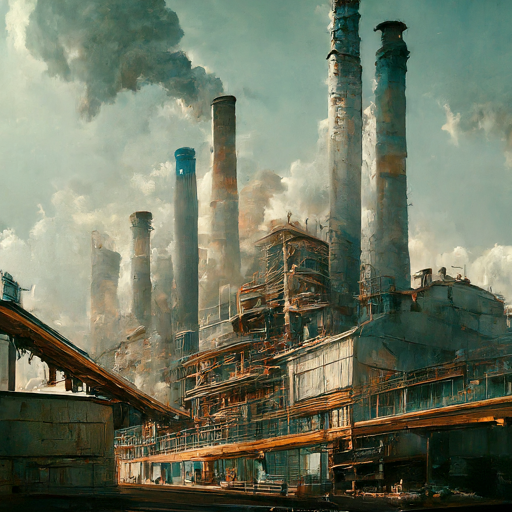
\includegraphics[width=4.5625in,height=\textheight]{images/industrial.jpeg}

\begin{itemize}
\item
  Overview of the industrial sector's importance in Pakistan's economy
\item
  Contribution to GDP, employment, and exports
\end{itemize}

\subsection{Contribution to the GDP}\label{contribution-to-the-gdp}

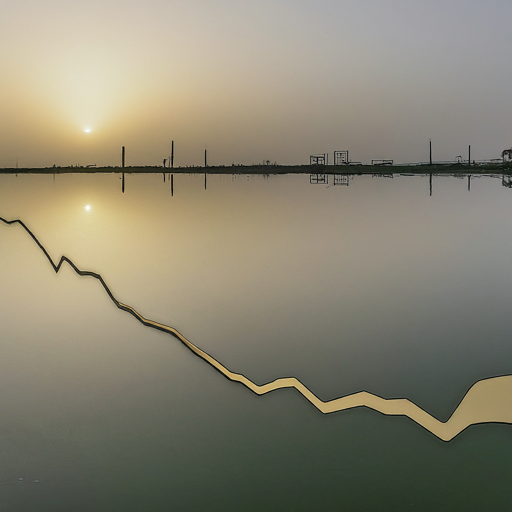
\includegraphics[width=4.5625in,height=\textheight]{images/industrial1.jpeg}

The industrial sector is a significant contributor to Pakistan's GDP. As
of 2023, it contributes approximately 22\% to the GDP. This sector plays
a vital role in job creation, foreign exchange earnings, and overall
economic development.

The industrial sector is a key driver of Pakistan's economy. It
contributes a significant portion to the GDP, creating jobs, generating
foreign exchange earnings, and fostering overall economic development.
The exact percentage contribution can fluctuate slightly year to year.

\subsection{Industrial Composition}\label{industrial-composition}

\begin{itemize}
\tightlist
\item
  Breakdown of industrial sub-sectors:

  \begin{itemize}
  \tightlist
  \item
    Manufacturing
  \item
    Mining and Quarrying
  \item
    Construction
  \item
    Utilities
  \end{itemize}
\end{itemize}

\subsection{Major Industries}\label{major-industries}

\begin{itemize}
\tightlist
\item
  Textile Industry: The largest and most important industry in Pakistan,
  accounting for a significant share of exports.
\item
  Cement Industry: A major player in the construction sector, catering
  to the domestic market and exporting to neighboring countries.
\item
  Food Processing Industry: A growing industry with immense potential,
  processing agricultural products like fruits, vegetables, and grains.
\item
  Pharmaceutical Industry: Producing a wide range of medicines and
  drugs, catering to domestic needs and exporting to other countries.
\item
  Automobile Industry: Assembling and manufacturing different types of
  vehicles, playing a crucial role in the transportation sector.
\end{itemize}

Speaker Notes Pakistan's industrial sector is diverse, with several
major industries contributing to the economy. The textile industry is
the largest and most important, accounting for a significant portion of
exports. Other significant industries include cement, food processing,
pharmaceuticals, and automobiles. These industries play a vital role in
fulfilling domestic needs and generating export revenue.

\subsection{Mining and Quarrying}\label{mining-and-quarrying}

\begin{itemize}
\tightlist
\item
  Overview of the sector's contribution
\item
  Major minerals:

  \begin{itemize}
  \tightlist
  \item
    Coal
  \item
    Natural gas
  \item
    Salt
  \end{itemize}
\end{itemize}

\subsection{}\label{section}

\subsubsection{Construction Sector}\label{construction-sector}

\begin{itemize}
\tightlist
\item
  Contribution to GDP and employment
\item
  Infrastructure projects driving growth
\item
  Challenges in project financing and regulatory environment
\end{itemize}

\subsubsection{Utilities}\label{utilities}

\begin{itemize}
\tightlist
\item
  Overview of electricity, gas, and water supply
\item
  Challenges in infrastructure development and distribution
\end{itemize}

\subsection{Challenges}\label{challenges}

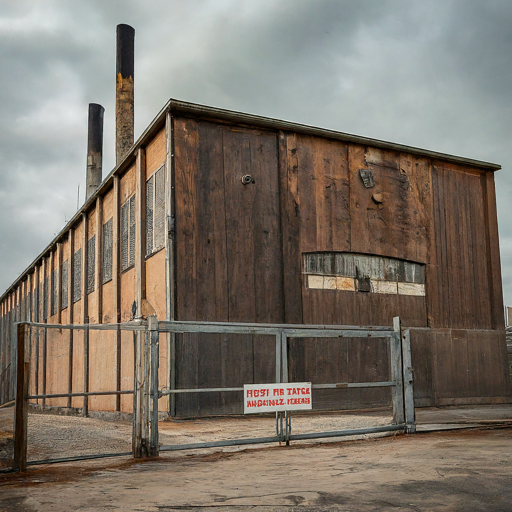
\includegraphics[width=4.5625in,height=\textheight]{images/industrial2.jpeg}

\subsection{Challenges Facing the Industrial
Sector}\label{challenges-facing-the-industrial-sector}

\begin{itemize}
\item
  Energy Shortage: A major challenge faced by the industrial sector,
  leading to production disruptions and increased costs.
\item
  Infrastructure Bottlenecks: Inadequate infrastructure, such as
  transportation and logistics networks, hinders smooth operations and
  increases costs.
\item
  Lack of Technological Advancement: The need for investment in modern
  technologies to improve efficiency and compete globally.
\item
  High Cost of Doing Business: Factors like complex regulations, high
  taxes, and corruption contribute to a challenging business
  environment.
\item
  Regulatory Hurdles: A complex regulatory environment that creates
  barriers to entry and compliance.
\item
  Skills Gap: A shortage of skilled labor and technical expertise.
\end{itemize}

Speaker Notes The Industrial sector of Pakistan faces several challenges
that hinder its growth. The chronic energy shortage disrupts production
and increases costs. Inadequate infrastructure, including transportation
and logistics networks, creates bottlenecks. The lack of investment in
modern technologies makes it difficult to compete globally.
Additionally, a complex regulatory environment, high taxes, and
corruption contribute to a high cost of doing business.

\section{Government Initiatives}\label{government-initiatives}

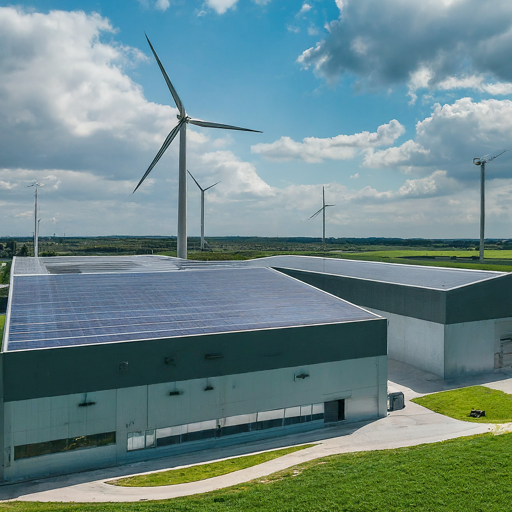
\includegraphics[width=6.66667in,height=\textheight]{images/industrial3.jpeg}

\subsection{Initiatives to Promote Industrial
Growth}\label{initiatives-to-promote-industrial-growth}

The government has launched several initiatives to promote industrial
growth:

\begin{itemize}
\item
  Development of Special Economic Zones (SEZs): Offering tax breaks,
  infrastructure facilities, and other incentives to attract investment.
\item
  Focus on Renewable Energy: Promoting renewable energy sources like
  solar and wind power to address the energy shortage.
\item
  Upgrading Infrastructure: Investing in infrastructure development to
  improve transportation and logistics networks.
\item
  Promoting Technology Adoption: Encouraging the adoption of modern
  technologies through incentives and skill development programs.
\end{itemize}

The government of Pakistan is aware of the challenges faced by the
industrial sector and has taken steps to address them. These initiatives
include developing Special Economic Zones, promoting renewable energy to
address the energy shortage, upgrading infrastructure, and encouraging
technology adoption through incentives and skill development programs.
The success of these initiatives will be crucial for the long-term
growth of the industrial sector.

\subsection{Opportunities for Growth}\label{opportunities-for-growth}

\begin{itemize}
\item
  Growing Domestic Market Demand: A large and growing population with
  increasing purchasing power.
\item
  Export Potential: Access to international markets and trade agreements
  with neighboring countries.
\item
  Technology Adoption and Innovation: Opportunities for modernization
  and efficiency improvement.
\item
  Investment Opportunities: Potential for foreign and domestic
  investment in various industries.
\end{itemize}

\subsection{Conclusion}\label{conclusion}

The industrial sector of Pakistan has the potential to be a significant
driver of economic growth. Addressing the challenges and leveraging the
opportunities will be crucial for realizing this potential.

Sure, here are slides based on the provided text:

\subsection{National Industrial
Policy}\label{national-industrial-policy}

\begin{itemize}
\tightlist
\item
  Title: Formulating a National Industrial Policy for Pakistan
\item
  Content: An Industrial Advisory Council, constituted by the federal
  government, is formulating the National Industrial Policy. The
  committee has articulated its vision of an export-led industrial
  development to take Pakistan's exports to \$100 billion within five
  years.
\end{itemize}

\begin{center}\rule{0.5\linewidth}{0.5pt}\end{center}

\textbf{Slide 2: Current Industrial Landscape} - Title: Appraisal of
Pakistan's Industrial Architecture - Content: An appraisal of Pakistan's
existing industrial architecture and its structural frailties is
essential. The current industrial structure has made Pakistan's economy
an outlier in a high-growth geographical region, despite being
surrounded by fast-growing economies such as China and India.

\begin{center}\rule{0.5\linewidth}{0.5pt}\end{center}

\textbf{Slide 3: Structural Dysfunction} - Title: Understanding
Structural Dysfunction - Content: Pakistan's imports of \$55.3 billion
were double its exports during FY 2022-23, with only a fraction of
imports used as inputs for export-oriented production. This indicates a
significant imbalance and highlights the structural dysfunction of
Pakistan's industrial sector.

\begin{center}\rule{0.5\linewidth}{0.5pt}\end{center}

\textbf{Slide 4: Rationale for Industrial Policy} - Title: Divergent
Views on Industrial Policy - Content: Economists have divergent views on
the rationale of a national industrial policy. While some argue for
market-led development, others point to successful examples like Japan,
South Korea, and Taiwan, which have used industrial policies
effectively.

\begin{center}\rule{0.5\linewidth}{0.5pt}\end{center}

\textbf{Slide 5: Industrial Distortions} - Title: Major Distortions in
Pakistan's Industrial Structure - Content: Pakistan's industrial
structure exhibits four major distortions, including an anti-export
bias, reliance on import substitution, market-seeking FDI, and policy
capture. These distortions hinder export-led growth and efficiency.

\begin{center}\rule{0.5\linewidth}{0.5pt}\end{center}

\textbf{Slide 6: Need for Radical Reforms} - Title: Instituting Radical
Reforms - Content: A forward-looking industrial policy needs to
institute radical reforms at both the structural and enterprise levels.
This includes transitioning from import substitution to export-led
growth and creating an enabling environment for new firms.

\begin{center}\rule{0.5\linewidth}{0.5pt}\end{center}

\textbf{Slide 7: Future Industrial Policy} - Title: Goals of a
Futuristic Industrial Policy - Content: A futuristic industrial policy
aims at creating a globally competitive industrial structure and
rewarding efficiency and productivity over lobbying skills. It
emphasizes the importance of self-sustaining industries and a gradual
transition to an innovation-driven economy.

\begin{center}\rule{0.5\linewidth}{0.5pt}\end{center}

\textbf{Slide 8: Challenges and Goals} - Title: Challenges and Goals -
Content: Developing an effective industrial policy faces challenges from
vested interests and maneuvering of policy forums. The vital goal is to
steer the transition towards an efficiency-driven export-led economy in
the medium term and innovation-driven in the long term.

\begin{center}\rule{0.5\linewidth}{0.5pt}\end{center}

\textbf{Slide 9: Conclusion} - Title: Conclusion - Content: Building a
globally competitive industrial structure requires strategic reforms and
a long-term vision. Despite challenges, the goal of achieving export-led
growth and innovation-driven economy remains paramount for Pakistan's
industrial development.

\begin{center}\rule{0.5\linewidth}{0.5pt}\end{center}

Feel free to adjust the content or design of the slides as needed! Let
me know if you need further assistance.



\end{document}
